% Template for ICIP-2019 paper; to be used with:
%          spconf.sty  - ICASSP/ICIP LaTeX style file, and
%          IEEEbib.bst - IEEE bibliography style file.
% --------------------------------------------------------------------------
\documentclass{article}
\usepackage{spconf,amsmath,graphicx}

%%%% my use package

\usepackage{cite}
\usepackage{amsmath,amssymb,amsfonts}
\usepackage{algorithmic}
\usepackage{graphicx,color}
\usepackage{textcomp}
\usepackage{bbm}
\usepackage{bm}
\usepackage{caption}
\usepackage{graphicx, subfig}
\usepackage {booktabs}
\usepackage {bm}
\usepackage[colorlinks,
            linkcolor=blue,
            anchorcolor=blue,
            citecolor=blue]{hyperref}
\usepackage{multirow}

% Example definitions.
% --------------------
\def\x{{\mathbf x}}
\def\L{{\cal L}}

% Title.
% ------
%\title{L-SNet: Combine Localisation and Segmentation by ROI Recalibration  }
\title{L-SNet: From region localization to scale invariant medical image segmentation } 
% Single address.
% ---------------
\name{Jiahao Xie, Sheng Zhang, Jianwei Lu$^{\star}$, Ye Luo$^{\star}$}
  
\address{ School of Software Engineering, Tongji University, China }
%
% For example:
% ------------
%\address{School\\
%	Department\\
%	Address}
%
% Two addresses (uncomment and modify for two-address case).
% ----------------------------------------------------------
%\twoauthors
%  {A. Author-one, B. Author-two\sthanks{Thanks to XYZ agency for funding.}}
%	{School A-B\\
%	Department A-B\\
%	Address A-B}
%  {C. Author-three, D. Author-four\sthanks{The fourth author performed the work
%	while at ...}}
%	{School C-D\\
%	Department C-D\\
%	Address C-D}
%
\begin{document}
%\ninept
%
\maketitle
%
\begin{abstract}
\vspace{-3pt}
Coarse-to-fine models and cascade segmentation architectures are widely adopted to solve the problem of large scale variations in medical image segmentation. 
However, those methods have two primary limitations: the first-stage segmentation becomes a performance bottleneck; the lack of overall differentiability makes the training process of two stages asynchronous and inconsistent. In this paper, we propose a differentiable two-stage network architecture to tackle these problems. In the first stage, a localization network (L-Net) locates Regions of Interest (RoIs) in a detection fashion; in the second stage, a segmentation network (S-Net) performs fine segmentation on the recalibrated RoIs; a RoI recalibration module between L-Net and S-Net 
eliminating the inconsistencies.
Experimental results on the public dataset show that our method outperforms state-of-the-art coarse-to-fine models with negligible computation overheads. 
%We will release the codes once the paper gets accepted.\par

% To solve the problem of large scale variations in medical image segmentation, widely used coarse-to-fine methods consist of two cascade segmentation models, in which one is for the region of interests (RoIs) localization and the other is for the segmentation. There are mainly two limitations of these methods: 1. Instead of detection, segmentation model is overused to predict the location of RoIs; 2. Few methods bridge two stages in an interpretable and differentiable way. In this paper, we propose a novel two-stage architecture L-SNet to address these problems. In the first stage, L-Net locates RoIs in a detection fashion. In the second stage S-Net performs fine segmentation on located RoIs. To eliminate the inconsistencies between two stages, RoI recalibration module is designed between L-Net and S-Net. Experimental results on the public Pancreas-CT dataset further validate that our method outperforms the state-of-the-art coarse-to-fine 
% methods with negligible computation overheads.

%To resolve the problem of large scale variations in medical image segmentation, widely used coarse-to-fine methods consist of two cascade segmentation models, decomposing the task to a localization task and a segmentation task. However, two problems remain unsolved: 1.segmentation model is overused to predict the localization of regions of interest 2. few methods bridge two stages in a interpretable and differentiable way. We present a novel two-stage architecture L-SNet to resolve those problems. In the first stage, L-Net locate RoIs in a detection fashion. In the second stage S-Net performs finer segmentation on located RoIs. To eliminate inconsistencies between two stages, RoI recalibration module is designed. Our method outperform the state-of-the-art coarse-to-fine model 0.79\% Dice Similarity Coefficients(DSC) with negligible computation overheads.


%we present a novel two-stage architecture L-SNet to resolve the problem of large scale variations in medical image segmentation. In the first stage, L-Net locate the regions of interest (RoIs) in an anchor free fashion. In the second stage S-Net performs finer segmentation on located RoIs. To eliminate inconsistencies between two stages, RoI recalibration module is designed. Our model can get precision segmentation in challenging dataset with  prodigious scale variance, and achieve 88.20\% Dice Similarity Coefficients(DSC) in TCIA pancreas segmentation dataset(Pancreas-CT) under 4-flod validation.

%In this paper, we propose an innovative two-stage architecture, L-SNet, to solve the problem of large scale variations in semantic segmentation. Our L-SNet is composed of first-stage L-Net, to locate regions of interests (RoIs), second-stage S-Net, to perform finer segmentation, and the RoI recalibration module, bridging those two stages and rendering L-SNet overall differentiable. Our method outperform the state-of-the-art coarse-to-fine model with negligible computation overheads and other powerful models, achieving 88.20\% Dice Similarity Coefficients (DSC) on TCIA pancreas segmentation dataset (Pancreas-CT), a challenging dataset with prodigious scale variances, based on 4-fold validation. Furthermore, the effectiveness of RR module, L-Net against U-Net as first-stage network, and joint optimization has been validated.
\end{abstract}
%
\begin{keywords}
medical image segmentation, scale variance, coarse-to-fine, anchor free detection.
\end{keywords}
%

%
% to do list:
% 1. 拆分KP BBR
% 2. ground-truth
% 3. 
%

\vspace{-12pt}
\section{Introduction}
\label{sec:introduction}
\vspace{-10pt}

Although various models have made significant achievements on the automated medical image segmentation \cite{unet,FCN,segnet,psp}, the important issue on scale variations remains unsolved, which is more salient in medical image processing since scales of different organs or lesions often vary prodigiously. Besides, proportions of the foreground objects on a whole image also vary greatly.
Currently, various research has been devoted to solving or mitigating these problems on the pancreas CT dataset (Pancreas-CT, available on TCIA\cite{TCIA}), on which the scale variation problem is especially obvious. \par

Recent researchers designed two-stage cascade models \cite{zhou2017fixed,3dc2f} to mitigate the scale imbalance in a coarse-to-fine way where the first model conducts coarse segmentation and roughly locate Region of Interests (RoIs), and the second model performs finer segmentation on the located RoIs. Although this approach has achieved state-of-the-art performance on the pancreas dataset, it suffers from a few limitations: inconsistencies between training and testing, difficulties in tuning, etc. 
% Though an improved model, RSTN \cite{RSTN} which is inspired by the coarse-to-fine models and embedded with a saliency transformation module to jointly optimize two deep networks, its optimization of locating RoIs is indirect and not easily interpretable. Further, the recurrent branch loads high computational complexities. 
% Attention U-Net\cite{attentionunet} alleviates the problem brought by large scale variations through the proposed attention gates, which merge both low-level and high-level features based on the global context of each. However, attention U-Net suffers from the low performance gain. Unlike all of them, our entirely-differentiable architecture L-SNet provides a solution to large scale variations and eliminates the limitations of the coarse-to-fine models. Fig.\ref{fig:intro} shows our improvements compare to coarse-to-fine method.\par
Though RSTN \cite{RSTN}, which is inspired by and improved the coarse-to-fine model with a saliency transformation module, can jointly optimize two deep networks, its optimization of locating RoIs is indirect and not interpretable. Further, the recurrent branch incurs high computational complexities. 
Attention U-Net \cite{attentionunet} alleviates the problem brought by large scale variations through the proposed attention gates, which merge both low-level and high-level features based on the global context of each. However, attention U-Net achieves a low performance gain. Unlike all of them, our entirely-differentiable architecture L-SNet solves large scale variations and eliminates many limitations of the coarse-to-fine models. Fig.\ref{fig:intro} shows our improvements compare to coarse-to-fine method. \par

% \begin{figure}[t]\vspace{-10pt}
%     \centering
%     \resizebox{0.48\textwidth}{!}{
%     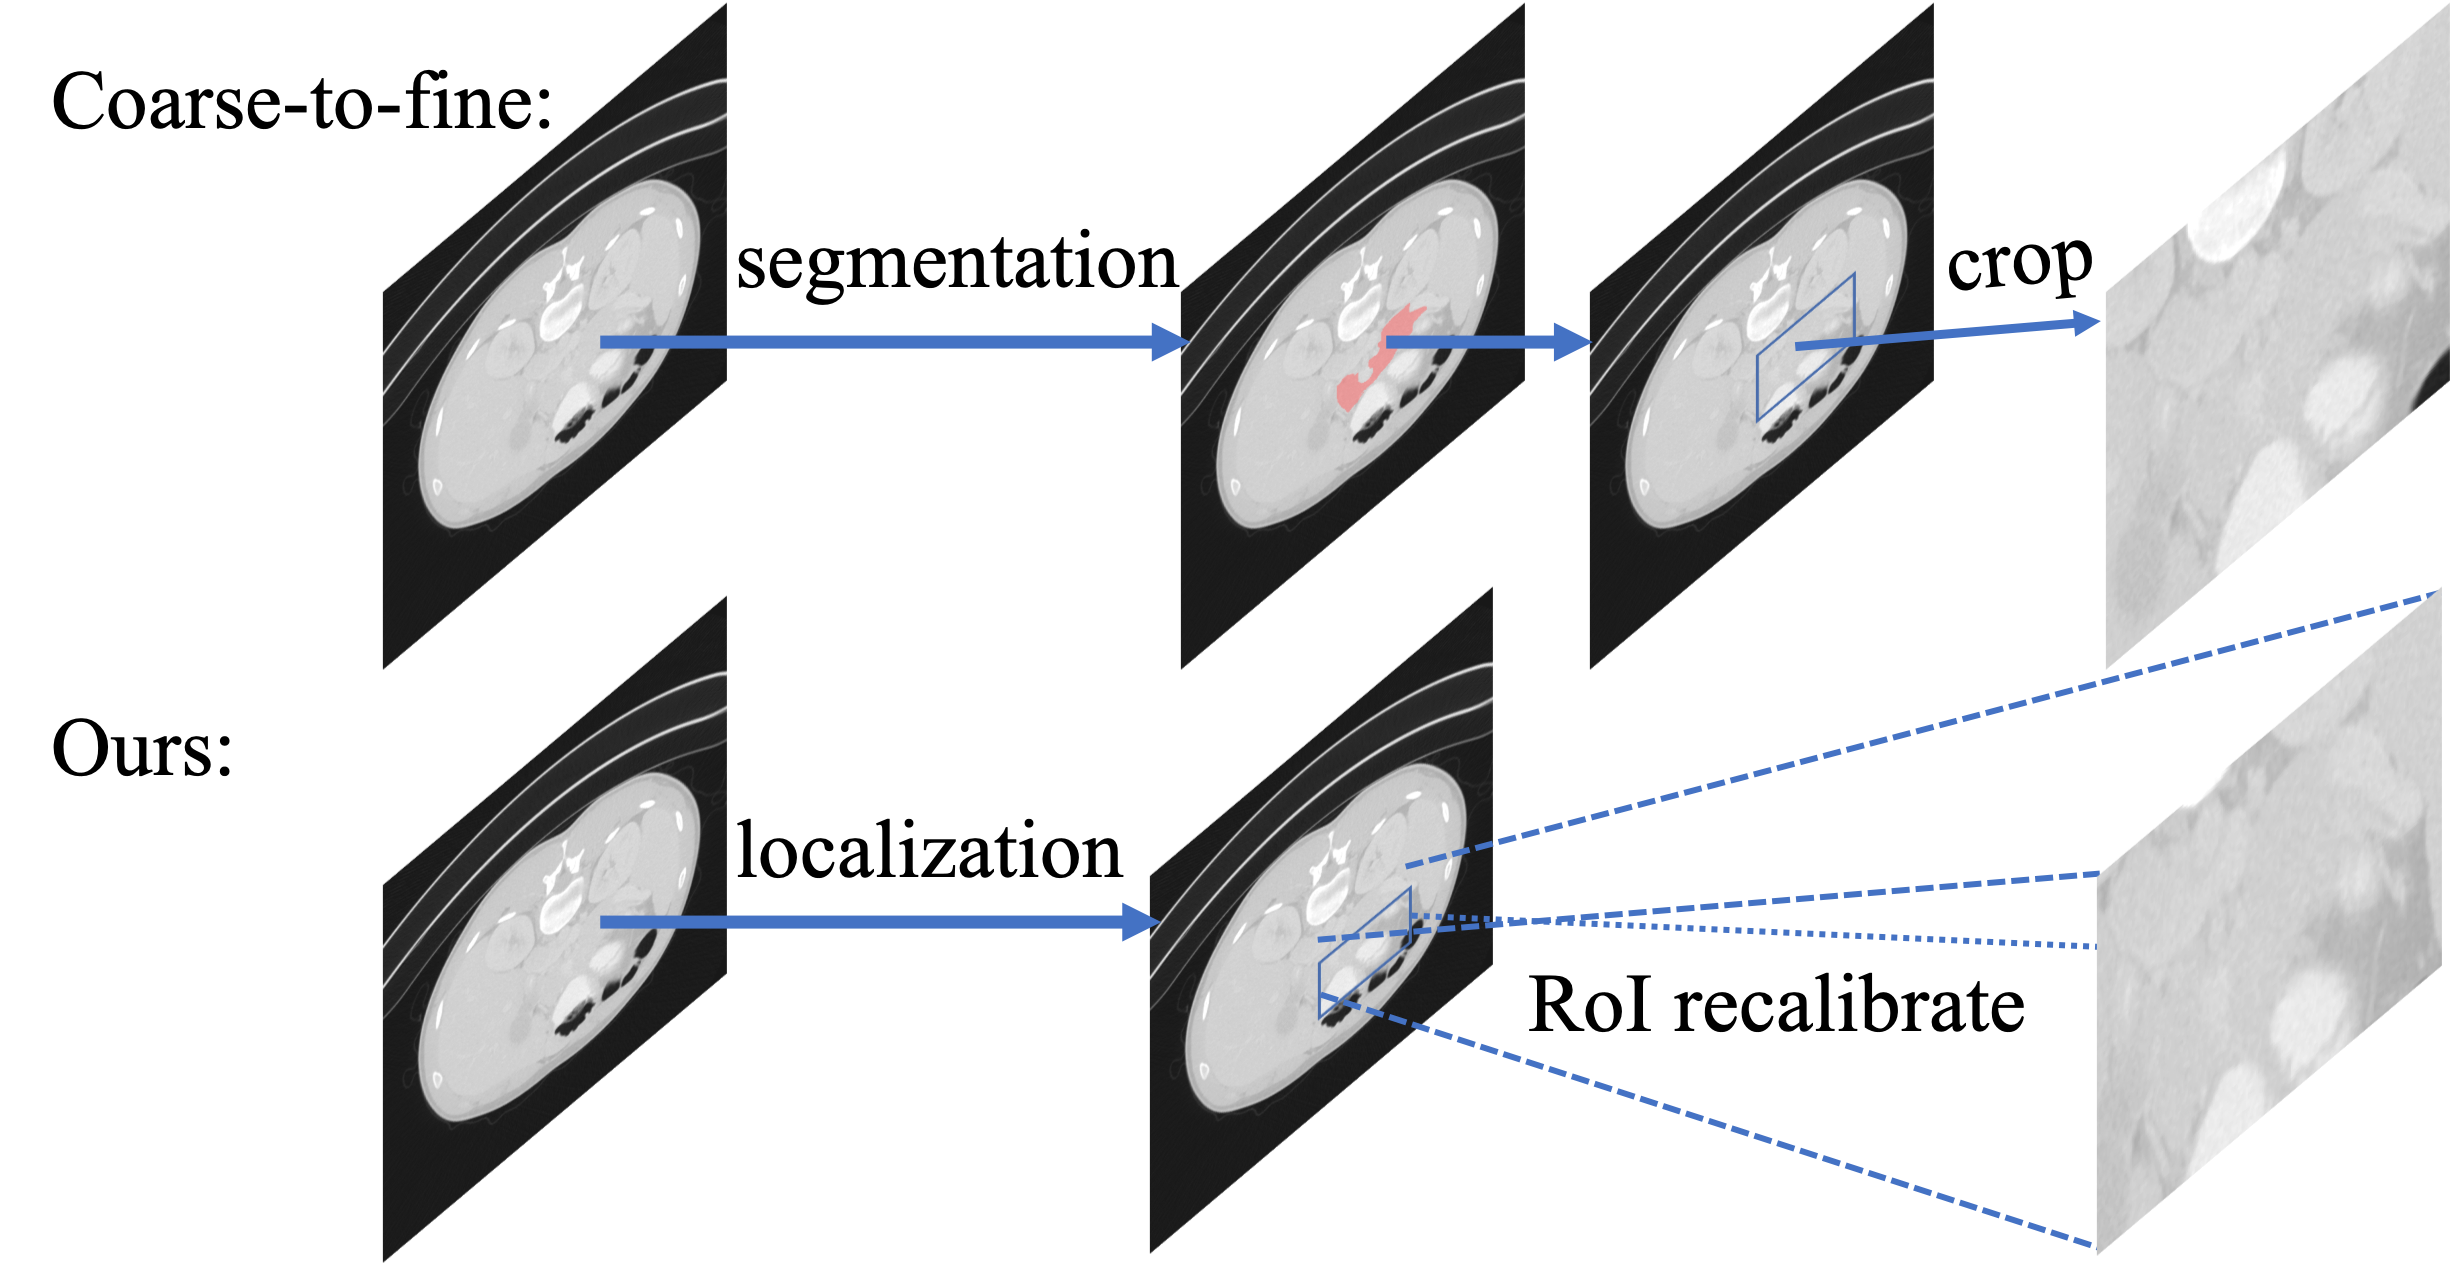
\includegraphics{intro.png}
%     }
%     \caption{Two representative samples exhibiting the large scale variations problem in TCIA Pancreas-CT dataset. The foregrounds can only occupied less than 2\% of a whole frame. Also, the pancreas's size in the right is about 20 times the size of that in the left.}
%     \label{fig:examples}\vspace{-22pt}
% \end{figure}
\begin{figure}[t]\vspace{-20pt}
    \centering
    \resizebox{0.45\textwidth}{!}{
    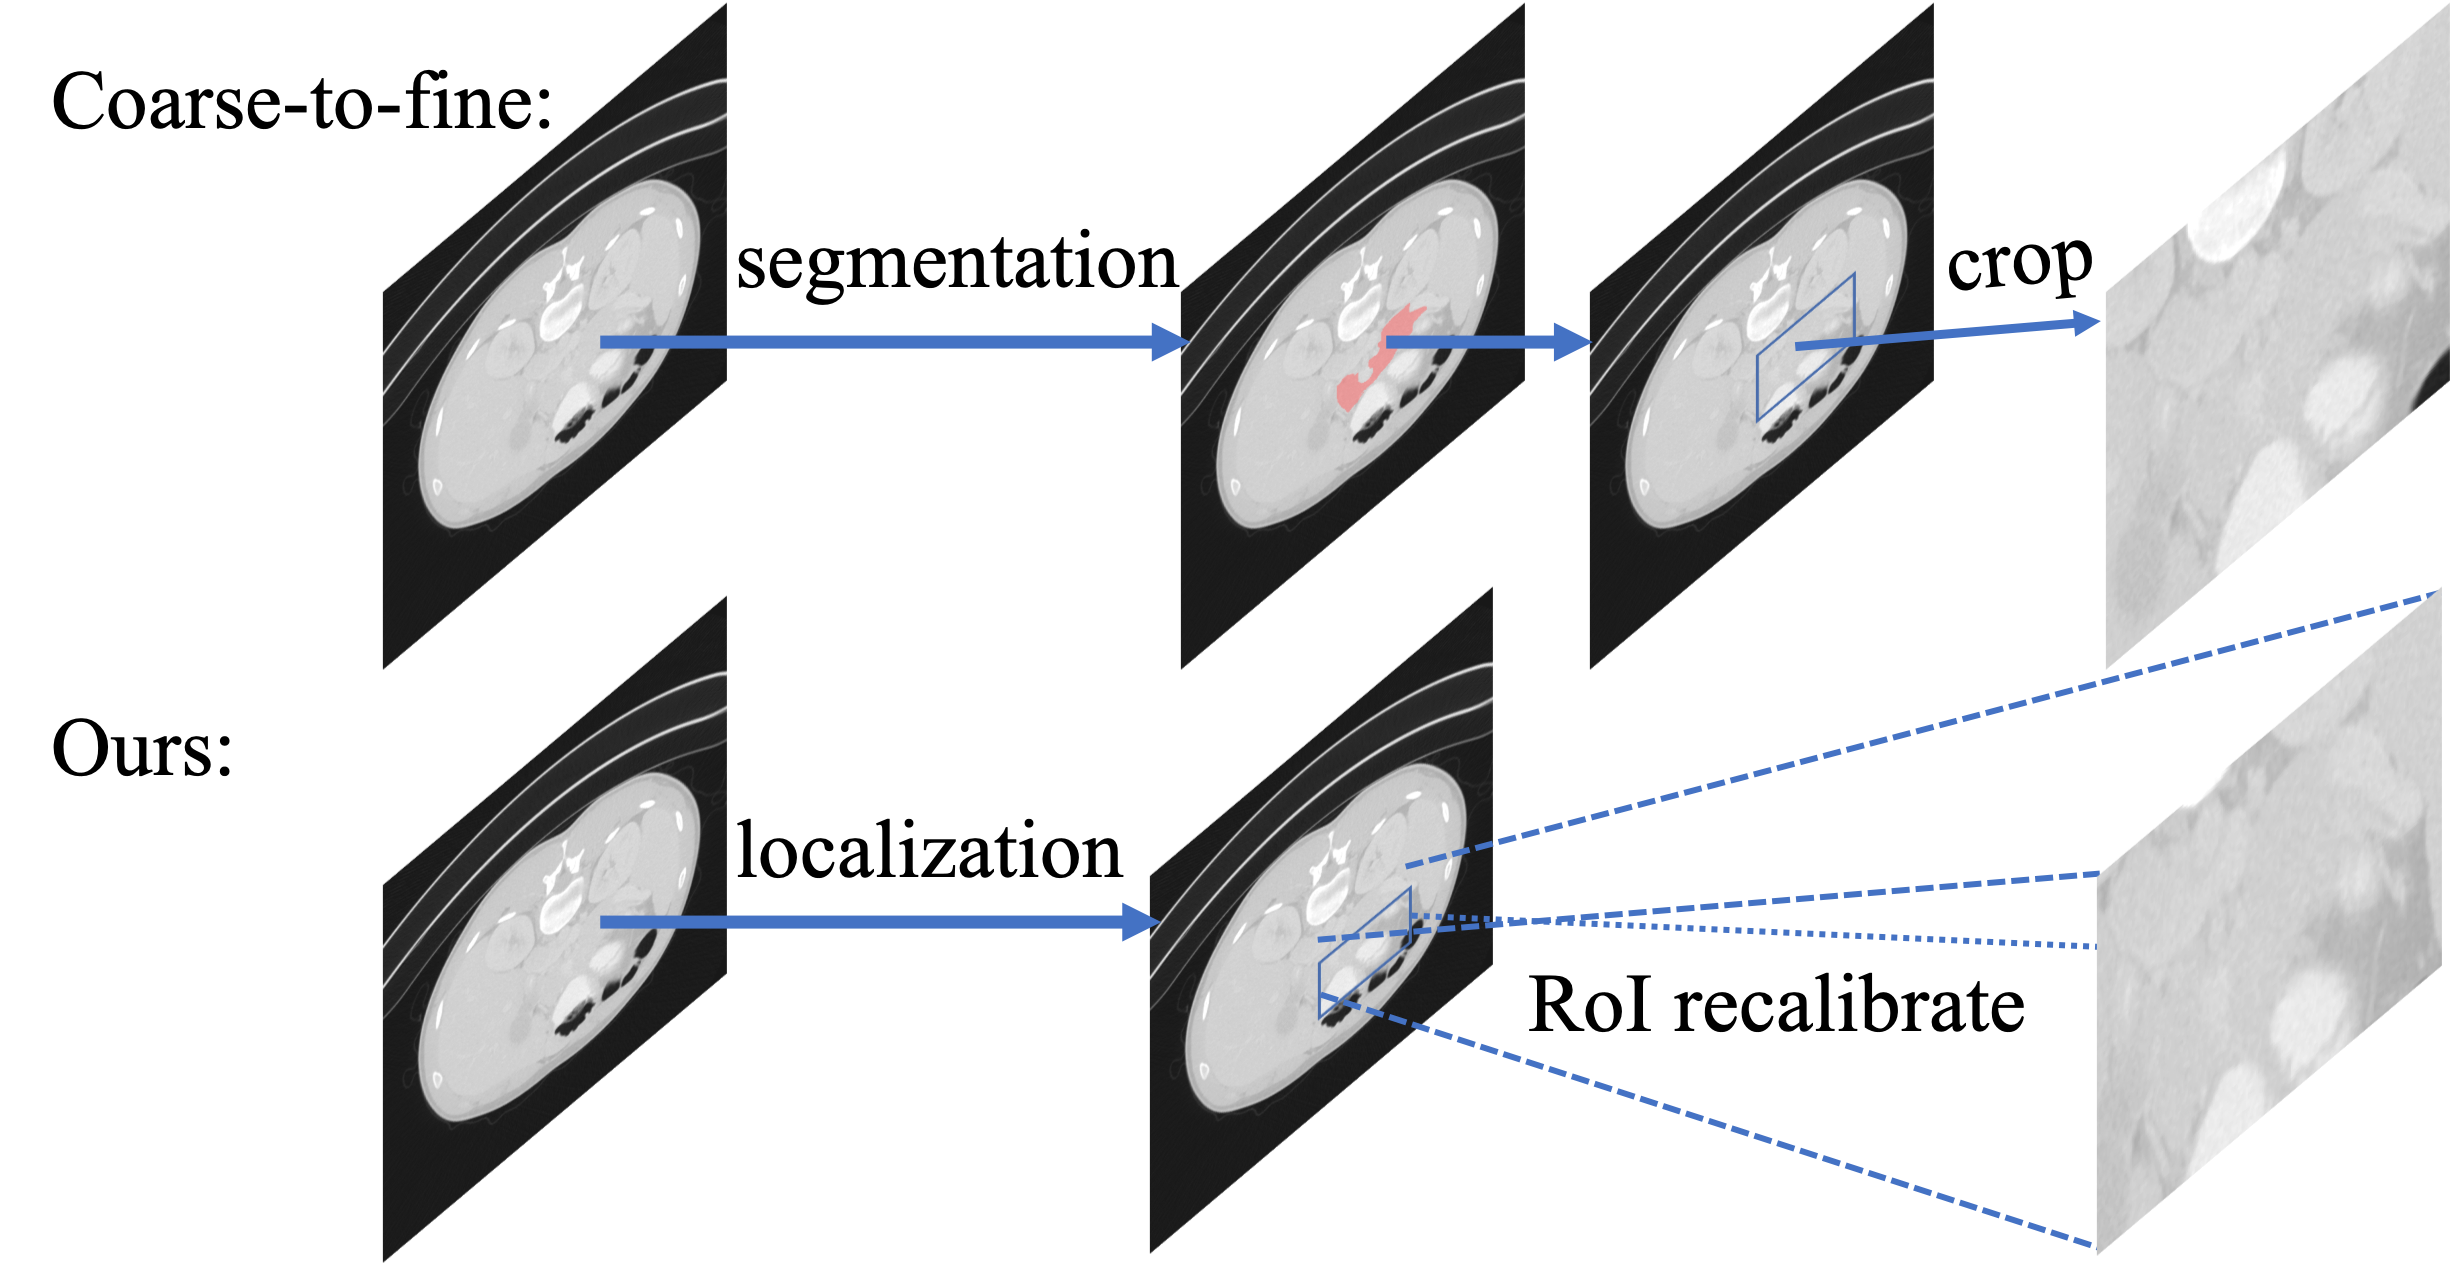
\includegraphics{intro.png}
    }\vspace{-10pt}
    \caption{The main difference between the widely used coarse-to-fine method and our L-SNet, before sending RoIs to the second stage for fine segmentation.}
    \label{fig:intro}\vspace{-15pt}
\end{figure}

\begin{figure*}[ht]\vspace{-10pt}
    \centering
    \resizebox{\textwidth}{!}{
    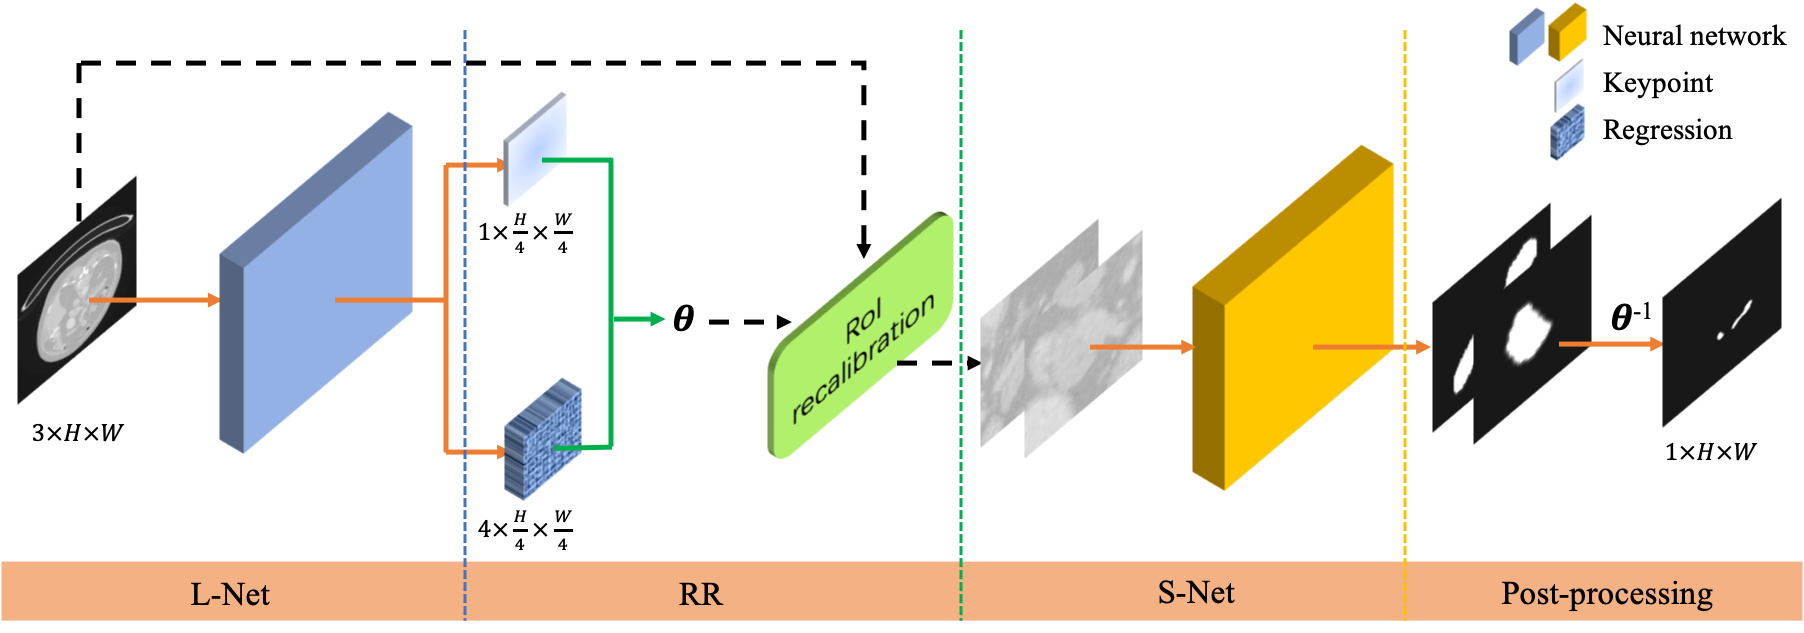
\includegraphics{L-SNet.png}
    }\vspace{-10pt}
    \caption{The overview of our proposed L-SNet. Given a CT image slice, L-Net is to locate RoIs, and the RoI recalibration module(RR) is to recalibrate located RoIs into a fixed scale for finer segmentation by S-Net. The post-processing is to restore finely segmented masks to their original shapes and positions on the input image. Our flexible architecture poses few restrictions on the form of L-Net and S-Net since they can be any CNNs.}
    \label{fig:process}\vspace{-10pt}
\end{figure*}


In this paper, we proposed an innovative two-stage network architecture, L-SNet, which uses L-Net to resolve the first location problem and use S-Net to perform the fine segmentation. As is shown in Fig.\ref{fig:process}, in the first stage, L-Net predicts and locates all RoIs; in the second stage, S-Net conducts finer segmentation; RoI recalibration module recalibrates RoIs, bridging two stages and making L-SNet entirely-differentiable. 
%We solve the problem of large scale variations by recalibration and overcome the weaknesses of most two-stage models (i.e., overall differentiability, joint optimization).
The main contributions of our work can be summarized as follows:
(1) We propose an innovative two-stage network architecture to solve the large scale variations, where the first stage conducts effective RoI detection rather than widely adopted coarse segmentation.
(2) We design an interpretable RoI recalibration module to bridge the gradients propagation between L-Net and S-Net, making L-SNet entirely differentiable. 
(3) Our proposed L-SNet consistently improves the coarse-to-fine models' performance on the Pancreas-CT dataset with measly computation overheads.
%%%%%%%%%%%%%%%%%%%%%%%%%%%%%%%%%%%%%%%%%%%%%%%%%5

\vspace{-15pt}
\section{The proposed methods}
\label{sec:the proposed methods}
\vspace{-10pt}
The overall architecture of our proposed method is displayed in Fig.\ref{fig:process}, which is mainly composed of three components: the localization Network (L-Net), the RoI Recalibration (RR) module, and the Segmentation Network (S-Net). 
Details of each component are introduced in the following sub-sections. \par

\vspace{-10pt}
\subsection{Localization Network}
\vspace{-5pt}
% location method involving 6 parameters
% degraded into two main tasks

L-Net locates each RoI using a bounding box (bbox) by predicting the location of its center point and the distances from that point to four boundaries of the box, which involves predicting six parameters---two for the center point's location $(x,y)$ and four for the distances $(l,r,t,b)$ from the center point to the left, right, top, and bottom edge of the bbox. This process can be decomposed into two tasks: keypoints prediction and distance regression. Therefore, the RoI can be accurately located by the bbox with a topleft anchor $(x-l,y+t)$ and a bottom right anchor $(x+r,y-b)$. \par

% Instead of predicting the anchor deviations as Faster-RCNN\cite{fasterrcnn} does, which has high complexities for computing anchors and intersection of union (IoU), or only predicting keypoints as CornerNet\cite{cornernet} does, which is anchor free but cuts off the gradient propagation when generating bounding boxes, we adopt the FCOS's method \cite{FCOS} where a keypoint position and its distances parameters $(l,r,t,b)$ are predicted for each foreground objects.

% To localize a RoI in an image which is actually a bounding-box region, there are at least six parameters: two for the center position $(x,y)$, four for the distances from the center to the left, bottom, top, and right edge of the bounding box $(l,b,t,r)$. With these six parameters, we can represent the four anchor points of the RoI, such as the top left anchor $(x-l,y+t)$ and the bottom right anchor $(x+r,y-b)$. L-Net, the most significant component in the proposed L-SNet, aims to locate all RoIs on an image by the detection of the key-points as the objects' centers and the regression of each center-to-boundary distance for precise size prediction of the bounding box.

\begin{figure}[t]\vspace{-5pt}
    \centering

    \resizebox{0.45\textwidth}{!}{
    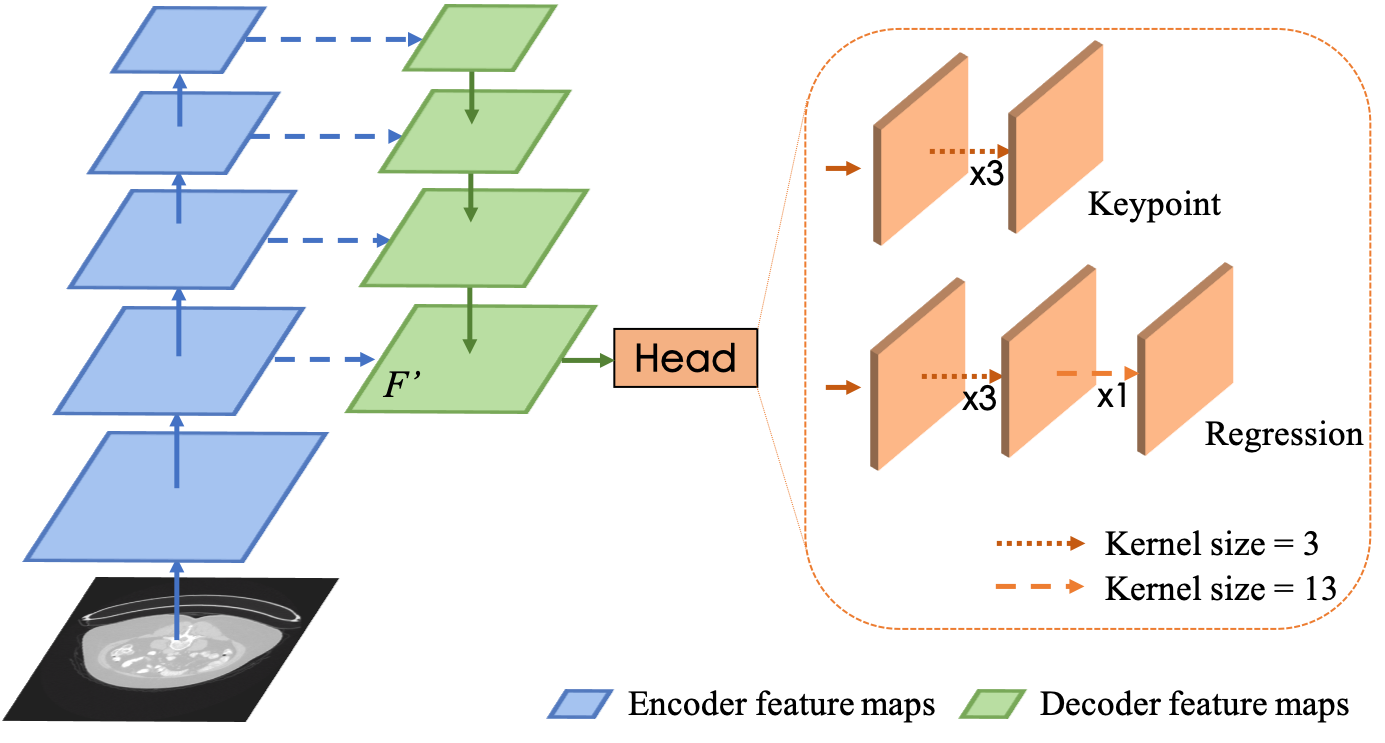
\includegraphics{L-Net.png}
    }\vspace{-10pt}
        \caption{The pipeline of L-Net. Feature map $F^{\prime}$ is extracted by a encoder-decoder structure. Two branches perform keypoints prediction and bounding box regression on $F^{\prime}$, respectively.}
    \label{fig:L-Net}\vspace{-15pt}
\end{figure}

\textbf{Network architecture.}
% overall architecture & input
% two output branches & two main tasks
% 2 branches structure
% mapping ?
Aiming to approximate the locations of foreground objects, we design the structure of L-Net as an encoder-decoder as most models do \cite{unet, deeplab, hourglass}. In practice, it can flexibly be any reasonable basic structure, such as FCN\cite{FCN} and U-Net\cite{unet}, with little modifications. \par

L-Net takes images with the size of $H \times W$ as input, and their RoIs are predicted and located in an anchor-free fashion by outputs of two branches: the keypoints prediction (KP) head, for locating each keypoint's position $(x,y)$, and the bounding box regression (BBR) head, for predicting distances $(l,r,t,b)$ for each keypoint. \par 

Taking the basic structure U-Net as an example (see Fig.\ref{fig:L-Net}), given the input, it is first sequentially down-sampled five times by the encoder to obtain a feature map with a size of $\frac{H}{32} \times \frac{W}{32}$, which is then upsampled three times by the decoder into a feature map $F^{\prime}$ with a size of $\frac{H}{4} \times \frac{W}{4}$. A center-aligned sampling strategy is adopted on the feature map $F^{\prime}$ so that each position $(x,y)$ can be mapped back to the position $(4x+2, 4y+2)$ on the input image.
\par

% The KP head outputs a tensor $K \in \mathbb{R}^{1 \times \frac{H}{4} \times \frac{W}{4}}$ containing keypoints positional information to approximate the ground-truth \bm{$K^*$}; 
% The BBR head outputs a tensor $T \in \mathbb{R}^{4 \times \frac{H}{4} \times \frac{W}{4}}$ encompassing distance information to approximate the ground-truth \bm{$T^*$}. 
% In KP head, we generate the result $K$ by three convolutions with kernel size 3 based on the feature map $F^{\prime}$. 
% In BBR head, we generate the result \bm{$T$} by two convolutions with kernel size 3 and one convolution with kernel size 13. The big kernel convolution have bigger receptive filed, which is better for regression task.
% The skip connections in L-Net are designed in a concatenation scheme. \par

% \subsubsection{center-aligned sampling and trace back}
% \label{subsec:sampling}
% The input image size, $320 \times 320$, different from the size of the target grid, we adopt the center-aligned sampling strategy when generating the heatmap $H^*$ and the regression target \bm{$T^*$}. In contrast, previous works \cite{fasterrcnn, yolo} adopt a left-top-aligned scheme but we argued that our center-aligned sampling is better in dense prediction tasks. \par

% Specifically, regarding each position $(x^*,y^*)$ on a source image, it is mapped to $(\frac{x^*}{s} , \frac{y^*}{s})$ on the target grid for generating the supervised data, heatmap $H^*$ and regression target \bm{$T^*$}; apropos each position $(x, y)$ on the target grid, it is mapped to $(xs+\frac{s}{2}, ys+\frac{s}{2})$ on the source image for locating RoIs. \par

% Different from the left-top-aligned sampling scheme in previous work \cite{fasterrcnn, yolo}, we adopt a center-aligned sampling strategy to locate RoIs on source images based on predicted bounding boxes.
%%%%%%%%%%%%%%%%

\textbf{Keypoints prediction.}
\label{subsec:keypoints-prediction} 
An ideal keypoint of the foreground object is its center point. Instead of computing the coordinates of the keypoints directly, in this paper, our KP head predicts keypoints by outputing a heatmap $ \bm{K} \in \mathbb{R}^{1 \times \frac{H}{4} \times \frac{W}{4}}$ to approximate the ground-truth heatmap $ \bm{K}^{*} \in \mathbb{R}^{1 \times \frac{H}{4} \times \frac{W}{4}}$ which is generated by the true centers of the foreground bboxes. In details, we use the ground-truth heatmap to guide another heatmap generation, and then locate keypoints on the generated heatmap by thresholding (Details in Section \ref{subsec:training-and-inference}).
Here, each element $K_{x,y}$ of $\bm{K}$ represents the output probability of the point $(x,y)$ being a foreground keypoint. %\par
%by three convolutions with kernel size 3 based on the feature map $F^{\prime}$ 
Each element $K^{*}_{x,y}$ of $ \bm{K}^*$, similar to \cite{duan2019centernet,cornernet}, is defined as:
\begin{align}
    \vspace{-5pt}
    K^*_{x,y} &= \min{(1, \sum_{(x_c,y_c) \in S}{e^{-\frac{d_x^2 + d_y^2}{2 \delta}}})}
    \vspace{-5pt}
\end{align}
\noindent where $d_x= \max{(0, |x - x_c|-\beta)}$, $d_y= \max{(0, |y - y_c|-\beta)}$. %
$S$ denotes the set of the center points of all foreground objects on $ \bm{K}^*$, and $(x_c, y_c)$ is the location of a center point in $S$. 
%${K}^{*}_{x,y}$ represents the distance of point $(x,y)$ to the object center, or
${K}^{*}_{x,y}$ represents  the probability of point $(x,y)$ to be a true keypoint. 
Here, the heatmap is generated in the form of Gaussian function with the variance $\delta$. $\beta$ controls its tolerant biases. We set $\delta=20$ by default and $\beta=2$ empirically. \par

\textbf{Bounding box regression.}
\label{subsec:bounding-box-regression}
Once the predicted key points are obtained, the BBR head predicts the bbox at the key point. Specifically, the BBR head regresses the $ \bm{T} \in \mathbb{R}^{4 \times \frac{H}{4} \times \frac{W}{4}}$ to approximate the ground-truth $\bm{T}^* \in \mathbb{R}^{4 \times \frac{H}{4} \times \frac{W}{4}}$. Here, each element ${T}_{x,y}$ of $\bm{T}$ represents the predicted values of $(l,r,t,b)$ at the point $(x,y)$. Each $ {T}^*_{x,y}$ on $ \bm{T}^*$ is a 4D vertor $(l^*,r^*,t^*,b^*)$ denotes the ground-truth point-edges distances of position $(x,y)$. 
%In other words, even though the predicted key point $(x,y)$ may be slightly different from the true object center $(x_c, y_c)$, we still can adjust $(l^*,r^*,t^*,b^*)$ to make the predicted bbox close to the ground-truth bbox. 
Later, we will show in our loss function that only the points located around the center of ground-truth bbox region have values of $ {T}^*_{x,y}$. We predict $ \bm{T}$ by two convolutions with kernel size 3 followed by one convolution with kernel size 13 based on the feature map $F^{\prime}$. The convolution with a larger kernel has larger receptive fields, which is more beneficial to the distance regression task. \par

%To guide this regression, each $ \bm{T}^*_{x,y}$ on $ \bm{T}^*$ is a 4D vertor $(l^*,r^*,t^*,b^*)$ denotes the left, right, top and bottom distance from location$(x, y)$ to the bounding box.

%To guide this regression, \bm{$T^*$} is generated where each 4-dim vector $T^{*}_{x,y}$ represents four distance regressand $(l,r,t,b)$ of position $(x,y)$ on \bm{$T^*$}. The ground-truth distance regressand is computed on input images and then is transformed into \bm{$T^*$}. 
% Furthermore, the predicted \bm{$T$} can provide the shape information for the 

% In our approach, the BBR head directly regresses four distances $(l,r,t,b)$ for each position.
% the bounding boxes at keypoints by predicting distances from keypoints to four edges of boxes to generate high quality RoIs. 
% That makes it possible to attain the transformation matrix for differentiable recalibration. \par

%Cooperating with the KP head, the BBR head can locate the bounding boxes on the target grid. In detail, each RoI can be located by one keypoint $(x,y)$, predicted by the KP head, and four parameters $(l,b,t,r)$, the distances between the keypoint and the left, bottom, top, and right edge of the bounding box (displayed in Fig.\ref{fig:bounding-box-regression}). Therefore, the top left anchor and the bottom right anchor are located in $(x-l,y+t)$ and $(x+r,y-b)$. \par
\vspace{-12pt}
\subsection{RoI recalibration}
\vspace{-5pt}

After RoIs with variant sizes are located, in order to feed S-Net with uniformized shapes of RoIs, a differentiable RoI Recalibration module (RR) is designed. Inspired by the grid generator in STN \cite{STN}, we design RR to recalibrate the located RoI by mapping each point $(x,y)$ on the RoI to a new position $(\Acute{x},\Acute{y})$ through an affine transformation which is defined as:
\vspace{-5pt}

\begin{equation}
    \left[
    \begin{matrix}
    \Acute{x} \\ \Acute{y}
    \end{matrix}
    \right]
   % = 
    %\mathcal{T}_\theta(
    %\left[
    %\begin{matrix}
    %x \\ y \\ 1
    %\end{matrix}
    %\right]
     = 
    \theta
    \left[
    \begin{matrix}
    x \\ y \\ 1
    \end{matrix}
    \right]
    =
\left[
    \begin{matrix}
    s_x & 0 & b_x \\
    0 & s_y & b_y 
    \end{matrix}
\right]
\left[
\begin{matrix}
x \\ y \\ 1
\end{matrix}
\right]
\end{equation}
where $\theta$ is the affine transformation matrix with parameters $\{s_x, s_y, b_x, b_y\}$. Here, $s_x$ and $s_y$ denotes scaling factors of $x$-axis and $y$-axis, and $b_x$ and $b_y$ are horizontal and vertical translations. 
%Once the localization of RoIs with variant sizes obtained, in order to uniformize shapes of RoIs to S-Net, a differentiable RoI Recalibration module (RR) is designed. Mathematically, given a predicted keypoint $(x,y)$ and its associated bbox regression result $(l,r,t,b)$, RR first converts them into four parameters $\{s_x, s_y, b_x, b_y\}$ as:
In order to back-propagate gradients, the four parameters $\{s_x, s_y, b_x, b_y\}$ are converted from the L-Net outputs (i.e., a keypoint $(x,y)$ and its associated bbox regression result $(l,r,t,b)$) as:
\vspace{-5pt}
\begin{align}
&s_x = \frac{l + r + \alpha}{W}, &b_x = x + \frac{r - l}{2} - \frac{W}{2}, \notag\\
&s_y = \frac{t + b + \alpha}{H}, &b_y = y + \frac{b - t}{2} - \frac{H}{2},
\label{f:totetha}\vspace{-5pt}
\end{align}
where $\alpha$ is the border margin of extra pixels padded around the localized RoIs, which is set as 15 in this paper.

It is worthy of remarking RR module's superiorities: coordinates are sampled and predicted in Float type in L-Net, and RR module sampled image by bilinear interpolation rather than hard cropping. So RR module eliminates the misalignment caused by quantization, overcoming weaknesses of the hard cropping in \cite{zhou2017fixed,RSTN}; the transformation matrix \bm{$\theta$} in RR module reasonably bridged L-Net and S-Net, which is more interpretable than dot multiplication in saliency transformation module \cite{RSTN}.
%satisfy any common transformation and is more interpretable than complex optimization in \cite{RSTN}. \par


% \begin{equation}
% \theta = 
% \left[
%     \begin{matrix}
%     s_x & 0 & b_x \\
%     0 & s_y & b_y
%     \end{matrix}
% \right]
% \end{equation}

% obtains the affine transformation parameter $\theta$ using the input proposal feature map, and recalibrates those proposals by $\theta$ into a uniform shape, $320 \times 320$, based on affine transformations including shifting and rescaling. Then the recalibrated RoIs forwarded to S-Net leverage further finer segmentation. \par

% The parameter of affine transformation $\theta$ to be learned by this module can be formulated as:
% \begin{equation}
% \theta = 
% \left[
%     \begin{matrix}
%     s_x & 0 & b_x \\
%     0 & s_y & b_y
%     \end{matrix}
% \right]
% \end{equation}
% \noindent where $s_x$ and $s_y$ denotes scaling factors of $x$-axis and $y$-axis, and $b_x$ and $b_y$ are horizontal and vertical translation distances. In practice, this $\theta$ is trained and output by a localisation network (i.e., multiple fc-layers) conditioned by the input RoI feature map.  \par

% Then the affine transformation $\mathcal{T}_\theta$ from point $(\Acute{x_i},\Acute{y_j})$ on the input RoI to point $(x_i^s, y_j^s)$ on the recalibrated feature map is written as:
% \begin{equation}
%     \left[
%     \begin{matrix}
%     x_i^s \\ y_j^s
    
%     \end{matrix}
%     \right]
%     = 
%     \mathcal{T}_\theta(\Acute{P}_{i,j}) = 
%     \theta \cdot 
%     \left[
%     \begin{matrix}
%     \Acute{x_i} \\ \Acute{y_j} \\ 1
%     \end{matrix}
%     \right]
%     =
% \left[
%     \begin{matrix}
%     s_x & 0 & b_x \\
%     0 & s_y & b_y 
%     \end{matrix}
% \right]
% \cdot
% \left[
% \begin{matrix}
% \Acute{x_i} \\ \Acute{y_j} \\ 1
% \end{matrix}
% \right]
% \end{equation}

\vspace{-10pt}
\subsection{Segmentation network}
\vspace{-5pt}
RoIs with an identical scale prepared, the S-Net can perform more accurate and finer segmentation on them, since a large proportion of backgrounds containing redundant or trivial information and interference of inconsistent scales have been removed. S-Net offers great flexibility in implementation, which, like L-Net, can be any basic structure. %we, in practice, take U-Net as a backbone.
% inverse transformation process
Specifically, S-Net takes as input a recalibrated RoI with size of $H \times W$, the same size as that of L-Net, and outputs its predicted mask $M$ to approximate the ground-truth $M^* \in \mathbb{R}^{\mathcal{C} \times H \times W}$, where $\mathcal{C}$ denotes the category number. 
\vspace{-10pt}
\subsection{Post-processing}
\label{subsec:post-processing}
\vspace{-2pt}
%In the post-processing, these masks are first transformed by the inverse transformation $\theta^{-1}$ into its original shape and then are placed to where their corresponding RoIs are originally located by L-Net (i.e., converted from masks of RoIs to masks of images) to form the final predicted image masks. \par 
All masks predicted by S-Net, they are first transformed by the inverse transformation $\theta^{-1}$ into their original sizes and locations to form their final predicted masks. Since $\theta$ is obtained in the RR, the inverse transformation $\theta^{-1}$ can be directly computed as:
\begin{equation}\vspace{-2pt}
    \theta^{-1}
    =
    \left[
    \begin{matrix}
    \frac{1}{s_x + \epsilon} & 0 & -b_x \\
    0 & \frac{1}{s_y + \epsilon} & -b_y 
    \end{matrix}
    \right].\vspace{-2pt}
\end{equation}
\noindent We add a smooth term $\epsilon=1e^{-7}$ in $\theta^{-1}$ to avoid the zero-division case.% though we have $\theta^{-1}\theta^T = I$ in theory. 

% \begin{table*}[t]
% \centering
% \caption{Main result.}
% \label{tab:mainresult}
% \setlength{\tabcolsep}{3mm}
% \begin{tabular}{p{3.8cm}lcccc}
% \hline\noalign{\smallskip}
%   Method & Dice Score & Precision & Recall & Dataset & Folds \\
% \noalign{\smallskip} \hline \noalign{\smallskip}
% U-Net\cite{unet}    & $0.8656\pm0.0101$  & $0.8960\pm0.0112$  & $0.9029\pm0.0046$ & CT-82 & 4-CV \\
% RSTN\cite{RSTN} $\dagger$   & $0.8450\pm0.0497$  & -  & -  & CT-82 & 4-CV  \\
% Attention U-Net\cite{attentionunet}$\dagger$   & $0.8310\pm0.0380$  & $0.8250\pm0.0730$  & $0.8400\pm0.0530$  & CT-82 + Ext & 4-CV  \\
% ResDSN C2F\cite{ResDSN}$\dagger$   & $0.8459\pm0.0486$  & -  & -  & CT-82 + Ext & 4-CV  \\
% ConResNet\cite{ConResNet}$\dagger$   & $0.8606\pm $-  & -  & -  & CT-82 & 4-CV  \\
% 3D Coarse-to-fine\cite{3dc2f}$\dagger$   & $0.8599\pm 0.0451$  & -  & -  & CT-82 & 4-CV  \\
% Attention U-Net\cite{attentionunet}    & $0.8688\pm0.0100$  & $0.8935\pm0.0070$  & $0.9101\pm0.0076$  & CT-82 & 4-CV  \\
% 2D Coarse-to-fine\cite{zhou2017fixed}$\dagger$ & $0.8237\pm 0.0568$  &  -  & -  & CT-82 & 4-CV  \\
% 2D Coarse-to-fine\cite{zhou2017fixed} & $0.8741\pm0.0136$  &  $0.9005\pm0.0085$  & $0.9136\pm0.0135$  & CT-82 & 4-CV  \\
% L-SNet (Ours) &  \bf{$0.8839\pm0.0134$}  & $0.9250\pm0.0086$  & $0.9045\pm0.0075$ & CT-82 & 4-CV \\
% \hline
% \end{tabular}
% \end{table*}

% \begin{table*}[t]
% \centering\vspace{-10pt}
% \caption{Performance comparison between our L-SNet and other state-of-the-art methods on TCIA Pancreas-CT dataset.}
% \label{tab:mainresult}
% \setlength{\tabcolsep}{3mm}
% \begin{tabular}{p{3.8cm}lccccc}
% \hline\noalign{\smallskip}
%   Method & Mean DSC(\%) & Max DSC(\%) & Min DSC(\%) & Dimension & Stages\\
% \noalign{\smallskip} \hline \noalign{\smallskip}
% %U-Net\cite{unet}    & $0.8656\pm0.0101$  & $0.8960$  & $0.9029$ & 2D \\
% RSTN\cite{RSTN}   & $84.50\pm4.97$  & $91.02$  & $62.81$ & 2D & two\\
% Attention U-Net\cite{attentionunet} & $83.10\pm3.80$  & -  & - & 2D & one\\
% Bayesian \cite{bayesian} & $85.32\pm4.19$  & 91.47  & 71.04 & 3D? & two\\
% ResDSN C2F\cite{ResDSN} & $84.59\pm4.86$ & $91.45$  & $69.62$ & 3D & two\\
% ConResNet\cite{ConResNet}  & $86.06 \pm  $ - & $92.00$  & $73.40$ & 3D & one?\\
% 3D Coarse-to-fine\cite{3dc2f} & $85.99\pm 4.51$ & $91.20$  & $57.20$ & 3D  & two\\
% %Attention U-Net\cite{attentionunet}    & $0.8688\pm0.0100$ & $0.8960$  & $0.9029$ & 2D \\
% 2D Coarse-to-fine\cite{zhou2017fixed} & $82.37\pm 5.68$ & $90.85$  & $62.43$ & 2D  & two\\
% \hline
% %Our baseline & $0.8741\pm0.0136$  & $0.8960$  & $0.9029$ & 2D  & two\\
% L-SNet (Ours) &  \bf{$88.20\pm0.98$}  & -  & - & 2D  & two\\
% \hline
% \end{tabular}\vspace{-10pt}
% \end{table*}


\vspace{-10pt}
\subsection{Implementation details}
\vspace{-5pt}
\label{subsec:implementation-details}
\textbf{Loss function.}
The loss function of the proposed L-SNet can be degraded into two parts: the loss of L-Net and the loss of S-Net. 
Compared with widely adopted BCELoss, our loss is designed to adapt to the large scale variations in segmentation tasks.
Noticeably, since our proposed architecture is entirely-differentiable, the loss of S-Net can also supervise L-Net. \par

Mathematically, the training objective is to simultaneously minimize the following two loss functions defined as:
\vspace{-14pt}
\begin{align}
    L_{L-Net} &= \frac{1}{N_l} \sum_{x,y \in l}{L_{cls}{(K_{x,y}, K_{x,y}^*)}}  \notag \\ 
    & +  \frac{\lambda}{N_l^+} \sum_{x,y \in l}{\mathbbm{I}{\{K_{x,y}^* \geq 0.5\}}L_{reg}{({T}_{x,y}, {T}_{x,y}^*)}} ,\\
    L_{S-Net} &= \frac{1}{N_s} \sum_{x,y \in s}{L_{cls}{(M_{x,y}, M_{x,y}^*)}}.
    \label{loss-l-net}
\end{align}
\vspace{-14pt}

Here $L_{cls}$ is a sum of the FocalLoss \cite{focalloss} and the DiceLoss weighted by 0.2. $L_{reg}$ is the DIoULoss \cite{DIoU}. 
$N_l, N_s$ denote the sample size for L-Net and S-Net, while $N_l^+$ refers to the positive sample size for L-Net.  $\mathbbm{I}{\{\cdot\}}$ denotes an indicator function, and we set $\lambda$ as 0.5 by default. \par
%$K_{x,y}$, $ \bm{T}_{x,y}$, and $M_{x,y}$ denote the position $(x,y)$ of L-Net's predicted heatmap \bm{$K$}, distance regressand \bm{$T$}, and segmentation mask $\bm{M}$ predicted by S-Net of the position $(x,y)$, respectively. The symbols of prediction targets are starred. $\mathbbm{I}{\{\cdot\}}$ denotes an indicator function, and we set $\lambda$ as 0.5 by default. \par

\textbf{Training and inference.}
\label{subsec:training-and-inference}
At the training stage, L-Net and S-Net are tuned alternatively. 
In each iteration of L-SNet, L-Net is first tuned by minimizing $L_{L-Net}$; then the RoI is located, recalibrated by RR module, and extracted, based on a randomly selected predicted keypoint of top three highest probability and its regression result; finally, L-SNet is tuned by minimizing $L_{S-Net}$ with the extracted RoI sent to S-Net. We decay gradients back-propagated from S-Net to L-Net by a factor $\gamma=0.1$, which attenuates S-Net's indirect supervision. \par
%%%%%%%%%%%%%%%%%%
At the inference stage, a test image is forwarded through S-Net, and the output predicted heatmap is activated (threshold by 0.5); then, centres of all activated connected components, as predicted keypoints, on that heatmap associated with their regressed distances can locate RoIs; S-Net conducts segmentation on these located RoIs and their final masks are obtained after being post-processed. \par

%%%%%%%%%%%%%%%%%%%%%%%%%%%%%
\vspace{-15pt}
\section{EXPERIMENTS}
\vspace{-10pt}
%this part elaborates our experimental results. \par
\subsection{Dataset and experimental settings}
\vspace{-5pt}
Experiments are conducted on TCIA Pancreas-CT dataset\cite{TCIA}, which contains 80 contrast-enhanced 3D CT scan with pancreas segmentation labelled in slice.
We take 2D image slices of 3D CT scan in the dataset as input (only use axial slices).
%In practice, we use ResNet18\cite{resnet} backbones for the first stage, L-Net, and ResNet34\cite{resnet} for our second stage. All backbones are pretrained on ImageNet\cite{imagenet}.
In practice, we use ResNet18\cite{resnet} backbones at the first stage, and ResNet34\cite{resnet} at the second stage. All backbones are pretrained on ImageNet\cite{imagenet}.
All models is optimized for 60 epochs by Adam optimizer with initial learning rate $r=1e^{-4}$. The learning rate decays by 0.1 each 25 epochs. We set $H=W=320$. The DSC and the mean IoU (mIoU) reported in Tables are the averaged score of all slices. mIoU is for the first stage, while DCS is for the second-stage. %of each model is the averaged score of 4-fold cross-validation results. \par


% To fairly compare our method with others, we do not fine tune our L-SNet carefully, but just apply hyper-parameters find under a U-Net with backbone ResNet34. In details, all models encoder are initialised by parameters trained under ImageNet, then trained by the Adam optimiser with learning rate set 0.0001, batch size set 16, step decay schedule are used by set learning rate decay to 1/10 after every 25 epoch, totally we trained 60 epoch. Limited to GPU memory, H and W set as 320.
% All result in ours experiments are mean scores under 4-fold cross-validation.

% \begin{table}[t]
% \centering\vspace{-10pt}
% \caption{Performance comparison between our L-SNet and other state-of-the-art methods on TCIA Pancreas-CT dataset.}
% \label{tab:mainresult}
% \setlength{\tabcolsep}{2.5mm}
% \begin{tabular}{p{3.25cm}lccc}
% \hline\noalign{\smallskip}
%   Method & Mean DSC & Max & Min\\
% \noalign{\smallskip} \hline \noalign{\smallskip}
% RSTN\cite{RSTN}   & $84.50\pm4.97$  & $91.02$  & $62.81$ \\
% Attention U-Net\cite{attentionunet} & $83.10\pm3.80$  & -  & - \\
% Bayesian \cite{bayesian} & $85.32\pm4.19$  & 91.47  & 71.04 \\
% ResDSN C2F\cite{ResDSN} & $84.59\pm4.86$ & $91.45$  & $69.62$ \\
% ConResNet\cite{ConResNet}  & $86.06 \pm  $ - & $92.00$  & $73.40$ \\
% 3D Coarse-to-fine\cite{3dc2f} & $85.99\pm 4.51$ & $91.20$  & $57.20$ \\
% 2D Coarse-to-fine\cite{zhou2017fixed} & $82.37\pm 5.68$ & $90.85$  & $62.43$ \\
% \hline
% L-SNet (Ours) &  \bf{$88.20\pm0.98$}  & -  & - \\
% \hline
% \end{tabular}\vspace{-10pt}
% \end{table}

\begin{table}[t]
\centering\vspace{-10pt}
\caption{Performance comparison between our L-SNet and other methods on TCIA Pancreas-CT dataset with two different basic structures, FCN and U-Net.}
\vspace{-10pt}
\label{tab:mainresult}
\setlength{\tabcolsep}{1.3mm}
\begin{tabular}{p{3cm}lccc}
\hline\noalign{\smallskip}
  Method & DSC(\%) & Precision(\%) & Recall(\%)\\
\noalign{\smallskip} \hline \noalign{\smallskip}
U-Net\cite{unet}    & 86.56  & 89.60  & 90.29\\
Attention U-Net\cite{attentionunet}    & 86.88 & 89.60  & 90.29 \\
Coarse-to-fine U-Net & 87.41  &  90.05  & \textbf{91.36} \\
\textbf{L-SNet} (U-Net) &  \textbf{88.20}  & \textbf{92.50}  & 90.45 \\
\hline
FCN\cite{FCN}    & 84.28  & 88.68  & 86.85\\
Coarse-to-fine FCN & 86.16  &  91.78  & 87.84 \\
\textbf{L-SNet} (FCN) &  \textbf{87.20}  & \textbf{92.60}  & \textbf{89.07} \\
\hline
\end{tabular}\vspace{-10pt}
\end{table}

\vspace{-15pt}
\subsection{Main result}
\vspace{-5pt}
Multiple existing powerful architectures proposed by other researches, evaluated on the same dataset and with the same evaluation metrics, are compared with our L-SNet.
%We do not apply model-specific optimal settings to L-SNet for fair comparisons. The 2D Coarse-to-fine, uses the same backbones as L-SNet; one-stage models use ResNet34 as backbones.
% We implement coarse-to-fine methods \cite{zhou2017fixed, 3dc2f} in a 2D version, in which do coarse segmentation and finer segmentation by two segmentation models and connect two stages by cropping the RoI with 30 extra pixels.
We implement coarse-to-fine methods \cite{zhou2017fixed, 3dc2f} in a 2D version, where two segmentation stage (coarse and fine) are connected by the RoI cropping with a 15-pixel border padding.
Two-stage models use the same backbones as L-SNet's; one-stage models use ResNet34 as backbones.
It can be observed in Table \ref{tab:mainresult} that L-SNet achieves higheset DSC regardless of different basic structures. Besides, two-stage methods are substantially accurate than one-stage methods. Importantly, L-SNets with FCNs and U-Nets still outperform their coarse-to-fine counterparts by 1.04\% and 0.79\% DSC, respectively. These all prove the effectiveness of our L-SNet architecture. \par
%It can be observed in Table \ref{tab:mainresult} that L-SNet always achieves higheset DSC. L-SNet outperforming Coarse-to-fine method by 0.79\% DSC under FCN structure, and is much better than one-stage method.
%It can be observed in Table \ref{tab:mainresult} that L-SNet achieves $88.20\%$ on Mean DSC, outperforming all other benchmarks on Pancreas-CT and exhibiting the lowest standard deviations which displays its robustness. \par

% \begin{table}[ht]\vspace{-5pt}
% \centering
% \caption{The effectiveness of different components of our proposed method. %The settings of six experiments with validated factors marked with a tick are listed in rows and their DSC results are in last column.
% }\vspace{-10pt}
% \label{tab:ablation}
% \setlength{\tabcolsep}{2mm}
% \begin{tabular}{cccccc}  
% \hline\noalign{\smallskip}
%   S-Net & Aug & Loss & L-Net & RR & DSC(\%)\\
% \hline
% \checkmark & & & & & 84.12\\
% \checkmark & \checkmark & & & & 84.69\\
% \checkmark & \checkmark & \checkmark &  &  & 86.51\\
% \checkmark & \checkmark & \checkmark & \checkmark & & 87.86\\
% \checkmark & \checkmark & \checkmark & \checkmark  & \checkmark & \textbf{88.20}\\
% \hline
% \end{tabular}
% \end{table}

\begin{table}[ht]\vspace{-8pt}
\centering
\caption{The effectiveness of different components of our method. %The settings of six experiments with validated factors marked with a tick are listed in rows and their DSC results are in last column.
}\vspace{-10pt}
\label{tab:ablation}
\setlength{\tabcolsep}{2mm}
\begin{tabular}{cccccc}  
\hline\noalign{\smallskip}
  S-Net & Loss & L-Net & RR & DSC(\%)\\
\hline
\checkmark & & & & 84.69\\
\checkmark  & \checkmark &  &  & 86.51\\
\checkmark  & \checkmark & \checkmark & & 87.86\\
\checkmark  & \checkmark & \checkmark  & \checkmark & \textbf{88.20}\\
\hline
\end{tabular}\vspace{-10pt}
\end{table}
\vspace{-15pt}
\subsection{Ablation study}
\vspace{-5pt}
We decompose the accomplishment of L-SNet into four dominant factors (see Table \ref{tab:ablation}) which are studied in ablation: S-Net, our loss function versus BCELoss, L-Net, and RR operation versus cropping. All experiments are performed on U-Net basic structure.%Four model settings are properly ordered. \par

%Three dramatic performance increases on CT-82 in Table \ref{tab:ablation} when adding Loss, L-Net, and RR can conclude: our specially designed loss in \ref{subsec:implementation-details} is more effective than BCELoss, improving about 1\% on DSC; the two-stage model is more powerful than a single segmentation network, improving over 1\%; RoI recalibration replacing cropping can further improve accuracies by 0.5\% benefiting from the better RoI location and transformation. Specifically, the architecture in the $4_{th}$ row is identical to the 2D Coarse-to-fine in \ref{tab:mainresult}, which means RR module can effectively improve that model. \par

\vspace{-10pt}
\subsection{Detection v.s. segmentation at the first stage}
\vspace{-5pt}
As is mentioned in Section \ref{sec:introduction}, in the coarse-to-fine method, the segmentation model at the first stage actually executing the detection task is not so efficient as the detection model. We conduct an experiment where U-Net is replaced by our L-Net at the first stage of the coarse-to-fine method \cite{zhou2017fixed,3dc2f}. As Table \ref{tab:landu} shows, both mIoU and final DCS are significantly improved when L-Net is utilized with only a negligible computation increase. %Therefore, L-Net, a first-stage detection network, rather than a segmentation nework is adopted for valid reasons.
%%%%%%%%%%%%%%%%%%%%%%%%%
\begin{table}[ht]
\centering \vspace{-5pt}
\caption{Comparison between L-Net and U-Net as the first-stage network in the coarse-to-fine method.} %Params means the number of model parameters (million unit). }
\vspace{-8pt}
\label{tab:landu}
\setlength{\tabcolsep}{2mm}
\begin{tabular}{cccc}  
\hline\noalign{\smallskip}
First stage    & mIoU(\%) & DCS(\%) & Params(M)\\ 
\hline
U-Net & 83.83 &  87.41 & \textbf{14.33}\\
L-Net & \textbf{86.58} &  \textbf{87.86} & 14.50\\
\hline
\end{tabular}
\end{table}
%%%%%%%%%%%%%%%%%%%%%%%%%%%%%%%%%%
\vspace{-20pt}
\subsection{The effect of decay factor }
\vspace{-5pt}
The decay factor $\gamma$ reflects the intensity of S-Net's supervision on L-Net. 
Table \ref{tab:gil} provides the comparison results when using U-Net as the basic structure. 
Although a larger $\gamma$ may degenerate the detection performance, it leads to a better final segmentation score and a smaller gap between the mIoU of training and validation. 
It also can be seen that though $\gamma=1$ achieves the smallest gap between training and validation, the final DSC is low. This phenomenon shows that the RR module works in a more complex way, not just to reduce the gap between training and validation. \par
%It also can be seen that a moderate decay $\gamma=0.1$ achieves the apex in DSC.It can be concluded that the supervision of S-Net on L-Net based on RR module can effectively improve the overall performance, and our method is very robust to its variations. \par
%%%%%%%%%%%%%%%%%%%
\begin{table}[ht]
\centering \vspace{-8pt}
\caption{The effect of the decay factor $\gamma$ on detection (mIoU) and segmentation (DSC) results. %mIoU is the first-stage metric for detection, and DCS is the second-stage metric for segmentation.
}
\label{tab:gil}\vspace{-10pt}
\setlength{\tabcolsep}{2mm}
\begin{tabular}{ccccc}  
\hline\noalign{\smallskip}
{$\gamma$}    & 0 & 0.01 & 0.1 & 1\\
\hline
mIoU in training & \textbf{92.03} & 88.09 & 88.24 & 86.84\\
mIoU in validation & \textbf{86.58} & 84.88 & 84.98 & 84.68 \\
DSC(\%) & 87.86 & 88.05 & \textbf{88.20} & 87.21 \\
\hline
\end{tabular}
\end{table}
%%%%%%%%%%%%%%%%%%%


% By using RoI recalibration, gradients generated by S-Net can back-propagate to L-Net. The gradients in L-Net should be set carefully, since loss of S-Net supervise L-Net in a potential way, and not optimize $\theta$ directly. Table \ref{tab:gil} shows the influences when reduce gradients of $L_{S-Net}$ with respect to L-Net by $\lambda$ times.

\vspace{-24pt}
\section{Conclusion}
\vspace{-8pt}
%In this paper, we are devoted to solving the problem of large scale variations in medical image segmentation task by proposing a new  network architecture, L-SNet. Our L-SNet is a two-stage method composed of L-Net, responsible for localisation of RoIs, and S-Net, designed for segmentation, both of which are bridged by the RR module enabling gradient propagation between them. The experiments concluded that, with all of them, L-SNet achieves the state-of-the-art result on benchmark dataset CT-82.

%In this paper, we propose an innovative, entirely-differentiable, and two-stage architecture for medical image segmentation, L-SNet, which is composed of L-Net, for localisation of RoIs, and S-Net, designed for segmentation, and interpretable RR module to recalibrate RoIs, enabling gradient propagation between two stages. The problem of large scale variations is solved and many weaknesses of coarse-to-fine models are eliminated. Our experiments manifest that L-SNet outperforms multiple powerful segmentation models and the effectiveness of RR module, the first stage of detection, and joint optimization has been attested.

In this paper, we analysed previous works on medical image segmentation and proposed a new architecture, L-SNet. In L-SNet, segmentation task undertaken by both L-Net and S-Net: L-Net is designed for localisation and S-Net is designed for segmentation. RR module connected L-Net and S-Net and establish the overall differentiability. Experiments show that every module in L-SNet, concluding L-Net, S-Net, and RR module, improved the final DSC. Conclusively, with all modules in L-SNet, we outperform coarse-to-fine methods consistently.
% In this paper, a new network is proposed to address the large scale variation problem in the segmentation task on medical images. Unlike previous methods which are not end-to-end trainable or 

\vspace{-15pt}
\section{Acknowledgments}
\label{sec:majhead}\vspace{-8pt}
This work was supported by the General Program of National Natural Science Foundation of China (NSFC) (Grant No. 61806147), and Shanghai Natural Science Foundation of China (Grant No. 18ZR1441200).

\bibliographystyle{IEEEbib}
\bibliography{strings,refs}

\end{document}
